\documentclass{article}

\usepackage{listings}
\usepackage{amsmath,amsfonts,amsthm,amssymb,amsopn,bm}
\usepackage[margin=.9in]{geometry}
\usepackage{graphicx}
\usepackage{url}
\usepackage[usenames,dvipsnames]{color}
\usepackage{fancyhdr}
\usepackage{multirow}
\newcommand{\field}[1]{\mathbb{#1}}
\newcommand{\1}{\mathbf{1}}
\newcommand{\E}{\mathbb{E}} 
\renewcommand{\P}{\mathbb{P}}
\newcommand{\R}{\field{R}} % real domain
% \newcommand{\C}{\field{C}} % complex domain
\newcommand{\F}{\field{F}} % functional domain

\newcommand{\T}{^{\textrm T}} % transpose

\def\diag{\text{diag}}

%% operator in linear algebra, functional analysis
\newcommand{\inner}[2]{#1\cdot #2}
\newcommand{\norm}[1]{\left\|#1\right\|}
\newcommand{\twonorm}[1]{\|#1\|_2^2}
% operator in functios, maps such as M: domain1 --> domain 2
\newcommand{\Map}[1]{\mathcal{#1}}
\renewcommand{\theenumi}{\alph{enumi}} 

\newcommand{\Perp}{\perp \! \! \! \perp}

\newcommand\independent{\protect\mathpalette{\protect\independenT}{\perp}}
\def\independenT#1#2{\mathrel{\rlap{$#1#2$}\mkern2mu{#1#2}}}
\newcommand{\vct}[1]{\boldsymbol{#1}} % vector
\newcommand{\mat}[1]{\boldsymbol{#1}} % matrix
\newcommand{\cst}[1]{\mathsf{#1}} % constant
\newcommand{\ProbOpr}[1]{\mathbb{#1}}
\newcommand{\grade}[1]{\small\textcolor{magenta}{\emph{[#1 points]}} \normalsize}
\date{{}}

\setlength\parindent{0px}

\begin{document}
\title{Homework \#0}
\author{\normalsize{CSE 546: Machine Learning}\\
\normalsize{Prof. Kevin Jamieson} \\
\normalsize{Student: Mitchell Vollger} \\
\normalsize{Collaborators: April Lo, Anna Minkina, David Read, Eliah Overbey} \\
\normalsize{Due: 10/4/18  11:59 PM}}
\maketitle


\section{Analysis}
{\color{blue}
1. \grade{1} A set $A \subseteq \R^n$ is \emph{convex} if $\lambda x + (1-\lambda) y \in A$ for all $x,y\in A$ and $\lambda \in [0,1]$.
A \emph{norm} $\|\cdot\|$ over $\R^n$ is defined by the properties:
i) non-negative: $\|x\|\geq 0$ for all $x \in \  R^n$ with equality if and only if $x=0$,
ii) absolute scalability: $\|a \, x\| = |a| \, \|x\|$ for all $a \in \R$ and $x \in \R^n$, iii) triangle inequality: $\|x+y\| \leq \|x\| + \|y\|$ for all $x,y \in \R^n$.
\begin{enumerate}
	\item Using just the definitions above, show that the set $\{ x \in \R^n : \|x\| \leq 1\}$ is convex for any norm $\| \cdot \|$.
	\item Show that $\left(\sum_{i=1}^n |x_i|^{1/2}\right)^2$ is or is not a norm.
\end{enumerate} 
}

Part a:
	\begin{align}
	   	\| \lambda x + (1-\lambda) y \| & \le \|\lambda x\| + \|(1-\lambda)y\| \text{ by iii}\\
	    & \le  |\lambda| \| x\| + |(1-\lambda)| \|y\| \text{ by ii}\\
	    & \le  \lambda \| x\| + (1-\lambda) \|y\| \text{ because $\lambda \in [0,1]$}\\
    	& \le  \lambda + (1-\lambda) \text{ because $\|x\| \le 1$}\\
        & \le 1 
	\end{align}
    Thus we have shown that $\lambda x + (1-\lambda) y \in A$ for all $x,y \in A$ for any norm.\\
	
Part b:
    Let $ x = (0,1)^T$ and $y=(1,0)^T$:
    \begin{align}
        \left(\sum_{i=1}^n |x_i+y_i|^{1/2}\right)^2 & = ((0+1)^{1/2} + (1+0)^{1/2})^2 \\
        & = 4
    \end{align}
    This is not less than or equal to:
    \begin{align}
        \left(\sum_{i=1}^n |x_i|^{1/2}\right)^2 + \left(\sum_{i=1}^n |y_i|^{1/2}\right)^2 & = (0^{1/2} + 1^{1/2})^2 + (1^{1/2} + 0^{1/2})^2\\
        & = 2
    \end{align}
    Thus $iii$ is not satisfied, so this is not a norm. \\
\newpage









{\color{blue}
2. \grade{1} For any $x \in \R^n$, define the following norms: $\|x\|_1 = \sum_{i=1}^n |x_i|$, $\|x\|_2 = \sqrt{\sum_{i=1}^n |x_i|^2}$, $\|x\|_\infty = \max_{i=1,\dots,n} |x_i|$. Show that $\|x\|_\infty \leq \|x\|_2 \leq \|x\|_1$.\\
}

Starting with showing:
\begin{align}
    \norm{x}_1 & \ge \norm{x}_2 \\
    \sum_{i=1}^n \|x_i\| & \ge  \sqrt{\sum_{i=1}^n |x_i|^2} \\
    (\sum_{i=1}^n \|x\|)^2 & \ge  \sum_{i=1}^n |x_i|^2
\end{align}
Proof by induction that the sum of squares is less than the square of sums:
Base cases: n = 1 is true because $(|x_1)^2| =  |x_1|^2 $. Case for n is 2:
\begin{align}
    ( |x_1| + |x_2|)^2 & \ge |x_1|^2 + |x_2|^2 \\
    |x_1|^2 + |x_2|^2 + 2|x_1||x_2| & \ge |x_1|^2 + |x_2|^2 \\
        2|x_1||x_2| & \ge 0\\
\end{align}
This value is always greater than zero so the second case is true. Now we assume that it is true for the $n^{th}$ case and prove it for $n+1$. 
Assume for n:
\begin{align}
    ( |x_1| + |x_2| + ... + |x_n|)^2 & \ge |x_1|^2 + |x_2|^2  + ... + |x_n|^2 \\
\end{align}
Prove for $n+1$: 
\begin{align}
    ( |x_1| + |x_2| + ... + |x_n| + |x_{n+1}|)^2 & \ge |x_1|^2 + |x_2|^2  + ... + |x_n|^2 + |x_{n+1}|^2 \\
    ( |x_1| + |x_2| + ... + |x_n|)^2 + |x_{n+1}|^2 + |x_{n+1}|(|x_1|^2 + |x_2|^2  + ... + |x_n|^2)  & \ge |x_1|^2 + |x_2|^2  + ... + |x_n|^2 + |x_{n+1}|^2 \\
    \text{Remove the part proven in the nth case} \\
    |x_{n+1}|^2 + |x_{n+1}|(|x_1|^2 + |x_2|^2  + ... + |x_n|^2)  & \ge  |x_{n+1}|^2 \\
   |x_{n+1}|(|x_1|^2 + |x_2|^2  + ... + |x_n|^2)  & \ge 0 \\
\end{align}
This is true because all the terms are positive. Thus $(\sum_{i=1}^n \|x\|)^2 \ge \sum_{i=1}^n |x_i|^2 $ and $\norm{x}_1 \ge \norm{x}_2$.
Now need to show that:
\begin{align}
    \norm{x}_2 & \ge \norm{x}_{\infty} \\
    \sqrt{\sum_{i=1}^n |x_i|^2} & \ge  \max_{i=1,\dots,n} |x_i| \\
    \sum_{i=1}^n |x_i|^2 & \ge  \max_{i=1,\dots,n} |x_i|^2  \\
    \sum_{i=1}^n |x_i|^2 - \max_{i=1,\dots,n} |x_i|^2 & \ge  0  \\
    \sum_{i=1, i\ne max}^n |x_i|^2 & \ge  0  
\end{align}
All these terms are positive thus summed together they are greater than or equal to zero. 
Thus we have shown that $\|x\|_\infty \leq \|x\|_2 \leq \|x\|_1$.\\

\newpage







{\color{blue}
3. \grade{1} For possibly non-symmetric $\mat{A}, \mat{B} \in \R^{n \times n}$ and $c \in \R$, let $f(x, y) = x^T \mat{A} x + y^T \mat{B} x + c$. Define $\nabla_z f(x,y) = \begin{bmatrix} \frac{\partial f(x,y)}{\partial z_1} & \frac{\partial f(x,y)}{\partial z_2} & \dots & \frac{\partial f(x,y)}{\partial z_n} \end{bmatrix}^T$.  What is $\nabla_x f(x,y)$ and $\nabla_y f(x,y)$? \\
}

First some definitions:
\begin{align}
    \nabla_x a^T x & = a \\
    \nabla_x x^T A x & = (A + A^T) x \\
\end{align}
Now getting $\nabla_x f(x,y)$:
\begin{align}
    \nabla_x f(x,y) & = (A+A^T)x + (y^TB)^T + 0 \\
    & = (A+A^T)x + B^Ty  \\
\end{align}
Now getting $\nabla_y f(x,y)$:
\begin{align}
    f(x,y) & = x^TAx + y^TB x + c \\
    & = x^T \mat{A} x + x^TB^Ty + c \text{, because it is s scalar term}\\
    \nabla_y f(x,y) & = 0 + (x^TB^T)^T +0  \\
    & = Bx  \\
\end{align}






\newpage

{\color{blue}
4. \grade{1} Let $\mat{A}$ and $\mat{B}$ be two $\R^{n\times n}$ symmetric
matrices. Suppose $\mat{A}$ and $\mat{B}$ have the exact same set of eigenvectors
$\vct{u}_1, \vct{u}_2, \cdots, \vct{u}_n$ with the corresponding
eigenvalues $\alpha_1, \alpha_2, \cdots, \alpha_{n}$ for $\mat{A}$, and
$\beta_1, \beta_2, \cdots, \beta_{n}$ for $\mat{B}$. Please write down
the eigenvectors and their corresponding eigenvalues for the following matrices:
\begin{enumerate}
\item $\mat{C} = \mat{A}+\mat{B}$
\item $\mat{D} = \mat{A} - \mat{B}$
\item $\mat{E} = \mat{A}\mat{B}$
\item $\mat{F} = \mat{A}^{-1}\mat{B}$ (\mbox{assume $\mat{A}$ is invertible})
\end{enumerate}
}
First some definitions:
\begin{align}
U & = (u_1, u_2 ... u_n) \\
    \Lambda_a & = diag(\alpha_1,\alpha_2...\alpha_n) \\
    \Lambda_b & = diag(\beta_1,\beta_2...\beta_n) \\
    A & = U\Lambda_aU^T\\
    B & = U\Lambda_bU^T 
\end{align}
Part a:
\begin{align}
    C = A + B & =  U\Lambda_aU^T +  U\Lambda_bU^T \\
    & =  U(\Lambda_aU^T +  \Lambda_bU^T) \\
    & =  U(\Lambda_a +  \Lambda_b)U^T \\
    & =  U\Lambda_{a+b}U^T \text{, where:  } \Lambda_{a+b} = \Lambda_a +  \Lambda_b
\end{align}
Thus the eigenvectors are unchanged, and the eigenvalues are the sum of the diagonals from the eigenvalue matrices (i.e. $\alpha_1 + \beta_1,\alpha_2 + \beta_2, ... \alpha_n + \beta_n $). \\

Part b: 
\begin{align}
    D = A - B & =  U\Lambda_aU^T -  U\Lambda_bU^T \\
    & =  U(\Lambda_aU^T -  \Lambda_bU^T) \\
    & =  U(\Lambda_a -  \Lambda_b)U^T \\
    & =  U\Lambda_{a-b}U^T \text{, where:  } \Lambda_{a-b} = \Lambda_a -  \Lambda_b
\end{align}
Thus the eigenvectors are unchanged, and the eigenvalues are the difference of the diagonals from the eigenvalue matrices (i.e. $\alpha_1 - \beta_1,\alpha_2 - \beta_2, ... \alpha_n - \beta_n $).  \\

Part c.
\begin{align}
    E = A*B & =  U\Lambda_aU^TU\Lambda_bU^T \\
    & =  U\Lambda_aI\Lambda_bU^T \\
    & =  U\Lambda_a\Lambda_bU^T \\
    & =  U\Lambda_{ab}U^T \text{, where: $\Lambda_{ab} = \Lambda_{a}  \Lambda_{b} $ }
\end{align}
Thus the eigenvectors are unchanged, and the eigenvalues are the product of the diagonals from the eigenvalue matrices (i.e. $\alpha_1 \beta_1,\alpha_2 \beta_2, ... \alpha_n \beta_n $).\\

Part d.
\begin{align}
    F = A^{-1}*B & =  U\Lambda_a^{-1}U^{-1}  U\Lambda_bU^T \\
    & =  U\Lambda_a^{-1} I\Lambda_bU^T \\
    & =  U\Lambda_a^{-1} \Lambda_bU^T \\
    & =  U\Lambda_{b/a}U^T \text{, where: $\Lambda_{ab} = \Lambda_{b} / \Lambda_{a} $ }
\end{align}
Thus the eigenvectors are unchanged. And because the inverse of a diagonal matrix is just the reciprocal of each value along the diagonal, the eigenvalues are just the division of the diagonals from the eigenvalue matrices (i.e. $\beta_1/\alpha_1 , \beta_2/\alpha_2, ...  \beta_n/\alpha_n $).\\



\newpage






{\color{blue}

5. \grade{1} A symmetric matrix $\mat{A} \in \R^{n \times n}$ is \emph{positive-semidefinite (PSD)} if $x^T \mat{A} x \geq 0$ for all $x \in \R^n$. 
\begin{enumerate} 
	\item For any $y \in \R^n$, show that $y y^T$ is PSD. 
	\item Let $X$ be a random vector in $\R^n$ with covariance matrix $\mat{\Sigma} =
\ProbOpr{E}[(X-\ProbOpr{E}[X])(X-\ProbOpr{E}[X])\T]$. Show that $\mat{\Sigma}$ is PSD. 
	\item Assume $\mat{A}$ is a symmetric matrix so that $\mat{A} = \mat{U} \diag(\alpha) \mat{U}^T$ where $\diag({\alpha})$ is an all zeros matrix with the entries of ${\alpha}$ on the diagonal and $\mat{U}^T \mat{U} = I$. Show that $\mat{A}$ is PSD if and only if $\min_i \alpha_i \geq 0$. (Hint: compute $x^T \mat{A} x$ and consider values of $x$ proportional to the columns of $\mat{U}$, i.e., the orthonormal eigenvectors).
\end{enumerate}
}

Part a:
\begin{align}
    x^T(yy^T)x & = (x^Ty) (y^Tx) \text{, both of these terms are the same scalar value so}\\
    & = c*c \\
    & = c^2 \ge 0 
\end{align}
Squared real values are always greater than zero so we have shown it is PSD.\\

Part b, let $E[x] =u $.
\begin{align}
    y^T\Sigma y & = y^T E[(x-u)(x-u)^T] y \\
    & =  E[y^T(x-u)(x-u)^T y]  \\
    & =  E[ ((x-u)^Ty)^T(x-u)^T y] \text{, each term is just the same scalar} \\
    & =  E[ c*c ] \\
    & = E[c^2] \ge 0 
\end{align}
Squared real values are always greater than zero so we have shown it is PSD.\\

Part c. 
\begin{align}
    x^TAx & = x^TU diag(\alpha)U^Tx \\ 
    & = (x^TU) diag(\alpha) (U^Tx) \\
    & = y^T diag(\alpha) y \text{, where: } y=(U^Tx)  \\
    & = \sum_{i=1}^n \lambda_i y_i^2
\end{align}
The the only way this is PSD is if all the values of labmda are positive. Because if anyone of them is negative you can imagine choosing a $y_i$ from some set $y$ such that the term $\lambda_{negative} y_i^2$ has greater absolute value than the rest of the sum making the overall sum negative. \\



\newpage





{\color{blue}

6. \grade{1} Let $X$ and $Y$ be real independent random variables with PDFs given by $f$ and $g$, respectively. Let $h$ be the PDF of the random variable $Z = X+Y$.
\begin{enumerate}
	\item Derive a general expression for $h$ in terms of $f$ and $g$
	\item If $X$ and $Y$ are both independent and uniformly distributed on $[0,1]$ (i.e. $f(x)=g(x)=1$ for $x \in [0,1]$ and $0$ otherwise) what is $h$, the PDF of $Z=X+Y$?
	\item For these given explicit distributions, what is $\P(X \leq 1/2 | X+Y\geq 5/4)$?
\end{enumerate}
}

Part a:
\begin{align}
    p(Z \ge z) & = P(X+Y \ge z) \\
    & = P(Y \ge z-x) \\
    & = \int_{-\infty}^{\infty} \int_{-\infty}^{z-x} f_{xy}(x,y) dy dx  \\
    & = \int_{-\infty}^{\infty} \int_{-\infty}^{z-x} f(x)g(y) dy dx  \text{, by independence}\\
    & = \int_{-\infty}^{\infty}  f(x) \int_{-\infty}^{z-x}g(y) dy dx \\
    & = \int_{-\infty}^{\infty}  f(x) G(z-x) dx \text{, where $G$ is the CDF of y}\\
    h(z) = \frac{d}{dz}(p(Z \ge z) ) & = \frac{d}{dz}  \int_{-\infty}^{\infty}  f(x) G(z-x) dx \\
    & =   \int_{-\infty}^{\infty}  f(x) \frac{d}{dz}(  G(z-x) ) dx \\
    & =   \int_{-\infty}^{\infty}  f(x) g(z-x) \frac{d}{dz}(z-x) dx \\
    & =   \int_{-\infty}^{\infty}  f(x) g(z-x) dx 
\end{align}
Part b:
\begin{align}
     h(z) & = \int_{-\infty}^{\infty}  f(x) g(z-x) dx 
\end{align}
But this must be split up into two cases, for z between 0 and 1 and z between 1 and 2. 
First between zero and one:
\begin{align}
     h(z) & = \int_{0}^{z}  f(x) g(z-x) dx \\
     & = \int_{0}^{z}  1*1 dx \\
     h(z) & = z \text{ for } z \in [0,1]
\end{align}

Now between one and two:
\begin{align}
     h(z) & = \int_{z-1}^{1}  f(x) g(z-x) dx \\
     & = \int_{z-1}^{1}  1*1 dx \\
     & =  x |_{z-1}^1 dx \\
     h(z) & = 2-z \text{ for } z \in (1,2]
\end{align}

These two equations plus $h(z)=0\text{ for } z \notin [0,2]$ define the PDF $h(z)$.\\


Part c:\\

Using Bayes rule:
\begin{align}
    %p(x\le 1/2 | x + y \ge 5/4) & = \frac{p(z\ge 5/4 | x\le 1/2) p(x\le 1/2)}{p(z\ge 5/4)} 
    p(x\le 1/2 | x + y \ge 5/4) & = \frac{p(z\ge 5/4, x\le 1/2) }{p(z\ge 5/4)} 
\end{align}
Calculating each term of that expression:
\begin{align}
    %p(x\le 1/2 ) & = 1/2, \\
    p(z \ge 5/4 ) & = \int_{5/4}^2 2-z dz \\
     & = 2z - 1/2z^2 |_{5/4}^2 \\
     & = 2 - 10/4 +25/32 \\
     & = 9/32
\end{align}
For the last term we know that $x \le 1 / 2$ and $z \ge 5/4$. \\
Note that if x is less than $1/2$, y must always be at least $3/4$ for z to be greater than $5/4$. 
Thus we can evaluate the joint pdf (plug in x+y for z) for $h(z)$ for $z > 1$ with these limits in mind.\\
\begin{align}
    %p(z\ge 5/4 , x\le 1/2) & = \int_{3/4}^{1} \int_{5/4-y}^{1/2} 2-(x+y) dx dy  \\
    %& = \int_{3/4}^{1} 2x - xy - 1/2x^2 |_{5/4-y}^{1/2} dy  \\
    %& = \int_{3/4}^{1} 1 - 1/2y - 1/8 - (2(5/4-y) - y(5/4-y) -1/2(5/4-y)^2) dy  \\
    %& = \int_{3/4}^{1} -y^2/2 + 3y/2 -27/32 dy  \\
    %& =  -y^3/6 + 3y^2/4 -27/32y |_{3/4}^{1}  \\
    %& = \frac{1}{48}
    p(z\ge 5/4 , x\le 1/2) & = \int_{3/4}^{1} \int_{5/4-y}^{1/2} 1 dx dy  \\
    & = \int_{3/4}^{1} x|_{5/4-y}^{1/2} dy\\
    & = \int_{3/4}^{1} y-3/4  dy\\
    & =  1/2y^2-3/4y |_{3/4}^{1}  \\
    & = 1/2 -3/4 - 9/32 + 9/16 \\
    & = \frac{1}{32}
\end{align}
Plugging 
in:
\begin{align}
    p(x\le 1/2 | x + y \ge 5/4) & = \frac{p(z\ge 5/4 , x\le 1/2) }{p(z\ge 5/4)} \\
    & = \frac{ 1/32   }{ 9/32 } \\
    & = \frac{1}{9}
\end{align}




\newpage



{\color{blue}

7. \grade{1} A random variable $X \sim \mathcal{N}(\mu, \sigma^2)$ is Gaussian distributed with mean $\mu$ and variance $\sigma^2$. Given that for any $a,b \in \R$, we have that $Y = aX + b$ is also Gaussian, find $a,b$ such that $Y \sim \mathcal{N}(0,1)$.\\
}
For any linear transformation of a Gaussian.
\begin{align}
    X & \sim N(\mu, \sigma^2) \\
    & \text{If $a,b \in \R$ and $Y = aX+b$ then,} \\
    Y  & \sim N(a\mu +b, a^2\sigma^2)
\end{align}
Thus we need to solve:
\begin{align}
    a^2\sigma^2 & = 1 \\
    a & = \frac{1}{\sigma}, \\
    \mu/\sigma + b & = 0 \\
    b & = - \frac{\mu}{\sigma}  \\
\end{align}

Thus $ a  = \frac{1}{\sigma}$ and $b  = - \frac{\mu}{\sigma}$. \\






\newpage





{\color{blue}

8. \grade{1} If $f(x)$ is a PDF, we define the cumulative distribution function (CDF) as $F(x) = \int_{-\infty}^x f(y) dy$.
For any function $g : \R \rightarrow \R$ and random variable $X$ with PDF $f(x)$, define the expected value of $g(X)$ as $\E[g(X)] = \int_{-\infty}^\infty g(y) f(y) dy$. For a boolean event $A$, define $\1\{ A \}$ as $1$ if $A$ is true, and $0$ otherwise. Thus, $\1\{ x \leq a \}$ is $1$ whenever $x \leq a$ and $0$ whenever $x > a$. 
Note that $F(x) = \E[\1\{X \leq x\}]$.
Let $X_1,\dots,X_n$ be \emph{independent and identically distributed} random variables with CDF $F(x)$. 
Define $\widehat{F}_n(x) = \frac{1}{n} \sum_{i=1}^n \1\{X_i \leq x\}$.
\begin{enumerate}
	\item For any $x$, what is $\E[ \widehat{F}_n(x) ]$?
	\item For any $x$, show that $\E[ ( \widehat{F}_n(x) - F(x) )^2 ] = \frac{F(x)(1-F(x))}{n}$
	\item Using part b., show that $\displaystyle\sup_{x \in \R} \E[ ( \widehat{F}_n(x) - F(x) )^2 ] \leq \tfrac{1}{4n}$. 
\end{enumerate}
}

Part a:
\begin{align}
    E[\Hat{F}_n(x)] &= E[1/n \sum_{i=1}^n \1 (X_i < x)] \\
    &= 1/n E[\sum_{i=1}^n \1 (X_i < x)] \\
    &= \frac{1}{n} n E[ \1 (X < x)] \\
    &= F(x) \\
\end{align}


Part b:\\
\begin{align}
    \E[ ( \widehat{F}_n(x) - F(x) )^2 ] & = \E[ ( \widehat{F}_n(x) - E[\widehat{F}_n(x)] )^2 ] \\
    & = Var(\widehat{F}_n(x)) \\
    & = Var( \frac{1}{n} \sum_{i=1}^n \1\{X_i \leq x\} ) \\
    & = \frac{1}{n^2} Var( \sum_{i=1}^n \1\{X_i \leq x\} ) \\
\end{align}
But $\1\{X_i \leq x\}$ describes a binomial draw so:
\begin{align}
   \E[ ( \widehat{F}_n(x) - F(x) )^2 ] & = \frac{1}{n^2} Var( B(n, F(x)) ) \\
    & = \frac{1}{n^2} n F(x)(1-F(x)) \text{, because Var(Bino(n,p))=np(1-p) } \\
    & = \frac{F(x)(1-F(x))}{n}  \\
\end{align}


Part c:\\
\begin{align}
    \frac{d}{dF(x)} \frac{F(x)(1-F(x))}{n} & = 1/n(1 - 2F(x)) \\
     1/n(1 - 2F_{max}(x)) & = 0 \\
    (1 - 2F_{max}(x)) & = 0 \\
    F_{max}(x) & = \frac{1}{2} 
\end{align}
Thus plugging in:
\begin{align}
    \displaystyle\sup_{x \in \R} \E[ ( \widehat{F}_n(x) - F(x) )^2 ] & \leq \frac{F_{max}(x)(1-F_{max}(x))}{n}\\
    & \leq \frac{1/2 *1/2}{n} \\
    & \leq \frac{1}{4n}
\end{align}






\newpage










{\color{blue}

\section{Programming}

9. \grade{2} Two random variables $X$ and $Y$ have equal distributions if their CDFs, $F_X$ and $F_Y$, respectively, are equal: $\sup_{x} |F_X(x) - F_Y(x)| = 0$. 
The central limit theorem says that the sum of $k$ independent, zero-mean, variance-$1/k$ random variables converges to a Gaussian distribution as $k$ goes off to infinity.  
We will study this phenomenon empirically (you will use the Python packages Numpy and Matplotlib). 
Define $Y^{(k)} = \frac{1}{\sqrt{k}} \sum_{i=1}^k B_i$ where each $B_i$ is equal to $-1$ and $1$ with equal probability.
It is easy to verify (you should) that $\frac{1}{\sqrt{k}} B_i$ is zero-mean and has variance $1/k$.
\begin{enumerate}
	\item For $i=1,\dots,n$ let $Z_i \sim \mathcal{N}(0,1)$. If $F(x)$ is the true CDF from which each $Z_i$ is drawn (i.e., Gaussian) and $\widehat{F}_n(x) = \frac{1}{n} \sum_{i=1}^n \1\{ Z_i \leq x)$, use the homework problem above to choose $n$ large enough such that $\sup_x \sqrt{\E[ (\widehat{F}_n(x)-F(x))^2 ]} \leq 0.0025$, and plot $\widehat{F}_n(x)$ from $-3$ to $3$. (Hint: use \texttt{Z=numpy.random.randn(n)} to generate the random variables, and \texttt{import matplotlib.pyplot as plt};\\ \texttt{plt.step(sorted(Z), np.arange(1,n+1)/float(n))} to plot).
	\item For each $k \in \{1, 8, 64, 512\}$ generate $n$ independent copies $Y^{(k)}$ and plot their empirical CDF on the same plot as part a. (Hint: you can use $\texttt{np.sum(np.sign(np.random.randn(n, k))*np.sqrt(1./k), axis=1)}$ to generate $n$ of the $Y^{(k)}$ random variables.)
\end{enumerate}
Be sure to always label your axes. 
Your plot should look something like the following (Tip: checkout \texttt{seaborn} for instantly better looking plots.)
}

\newpage

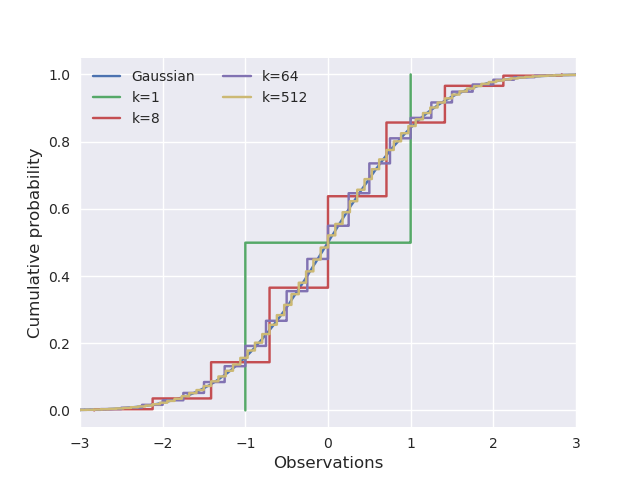
\includegraphics[width=4in]{problem9.png}

\lstinputlisting[language=python]{hw0.py}


\end{document}

